\section{Proxy}

O padrão Proxy adiciona uma camada de acesso 
a um objeto, fazendo com que qualquer interação 
com o objeto Proxy seja controlada antes de ser 
repassada para o objeto real. Existe mais 
de uma motivação para seu uso, apesar 
da estrutura do padrão, 
apresentada na figura \ref{proxy_struct},  
permanecer a mesma. Essas motivações 
podem ser divididas em três grupos de 
proxy: remoto, virtual e de proteção. 

Um proxy remoto pode ser utilizado como um 
representante de um objeto, servindo como um 
intermediário e armazenando dados que devem 
ser repassados para o objeto real. Já um 
proxy virtual armazena informações sobre 
um objeto de forma que ele possa ser criado 
apenas quando for necessário, economizando 
espaço ou tempo de execução. Por fim, um 
proxy de proteção pode controlar o acesso 
a um objeto, exigindo que um objeto cliente 
precise cumprir algum requisito antes de 
acessar o objeto real. 

\begin{figure}[htb]
	\caption{\label{proxy_struct}Estrutura do Proxy}
	\begin{center}
	    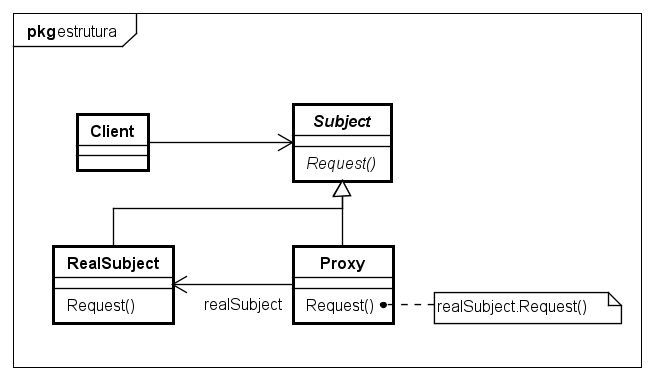
\includegraphics[scale=0.5]{5_padroes-contexto-funcional/5.2_estruturais/5.2.7_proxy/proxy_estrutura.png}
	\end{center}
\end{figure}

\subsection*{Exemplo Orientado a Objetos}

Como exemplo de Proxy podem ser utilizadas 
imagens que são incluídas em editores de 
texto. É desejado que um documento seja aberto 
rapidamente e o carregamento das imagens 
presentes nele pode causar uma lentidão 
desnecessária. Para isso, é criado um objeto 
Proxy que armazena em seus atributos as 
informações necessárias, como o caminho 
para a imagem e seu posicionamento no 
documento. Quando o documento termina de 
ser aberto, as imagens são carregadas de 
fato através de seus proxys. Esse é um 
exemplo de proxy virtual, seu diagrama de 
classes pode ser visto na imagem \ref{proxy_exemplo} 
e a implementação no código \ref{ooproxy}.

\begin{figure}[htb]
	\caption{\label{proxy_exemplo}Exemplo de Proxy}
	\begin{center}
	    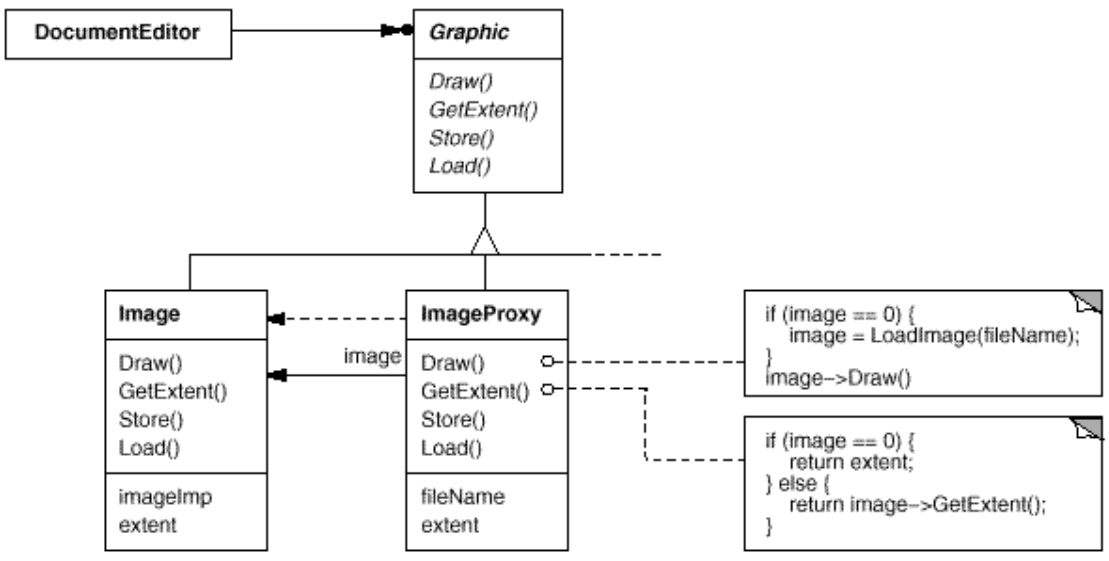
\includegraphics[scale=0.5]{5_padroes-contexto-funcional/5.2_estruturais/5.2.7_proxy/proxy_exemplo.png}
	\end{center}
\end{figure}

\begin{lstlisting}[caption={Proxy Orientado a Objetos},label=ooproxy]

trait Graphic {
  def Draw(point : Point)
  def GetExtent() : Point
  def Store(ostream : Stream[Byte])
  def Load(istream : Stream[Byte])
}

class Image (private val filename : String) extends Graphic {

  private var extent : Point = new Point

  def Draw(point: Point): Unit = {
    //Desenha imagem na tela
  }

  def GetExtent(): Point = extent

  def Store(ostream: Stream[Byte]): Unit = {
    //Salva imagem em um arquivo
  }

  def Load(istream: Stream[Byte]): Unit = {
    //Carrega imagem de um arquivo
  }
}

class ImageProxy(var filename : String, var extent : Point) extends Graphic {

  private var image : Image = null

  override def Draw(point: Point): Unit = {
    if(image == null){
      image = new Image(filename)
    }
    image.Draw(point)
  }

  override def GetExtent(): Point = {
    if(image==null){
      image = new Image(filename)
    }
    image.GetExtent()
  }

  def Store(ostream: Stream[Byte]): Unit = {
    //Salva imagem em um arquivo
  }

  def Load(istream: Stream[Byte]): Unit = {
    //Carrega imagem de um arquivo
  }
}

\end{lstlisting}

\subsection*{Contexto Funcional}

Para implementar um Proxy, uma função do 
editor de documentos pode receber como 
parâmetro uma função cuja assinatura seja 
a mesma do método Draw no exemplo orientado 
a objetos. Dessa forma, tanto é possível 
receber a função real quanto a função 
intermediária, sem que a função cliente 
esteja ciente de qual está sendo utilizada. 
A função intermediária, assim como nos 
métodos da classe intermediária no exemplo 
orientado a objetos, executará a função 
real, de acordo com o tipo de proxy que 
deve ser implementado. 

No código \ref{fpproxy}, a função intermediária 
DrawImageProxy, definida na linha 6, chama a 
função real DrawImage, definida na linha 2. 
A função EditorFunction, definid na linha 11, 
representa uma função cliente qualquer que 
precisa desenhar a imagem. Ao invés de chamar 
diretamente a função DrawImage, ela recebe 
como parâmetro uma função com a mesma assinatura, 
para que seja possível que ela receba a função 
Proxy.

Existem algumas desvantagens quanto a essa 
implementação. Não é possível que haja 
estado atrelado ao Proxy, pois para que 
esse estado seja refletido na função 
cliente, é necessário que uma nova função, 
atualizada com o novo estado do Proxy, seja 
retornada pelas funções intermediárias. 
Isso faz com que o cliente precise gerenciar 
a mudança do Proxy, violando 
um dos propósitos do padrão. 

\begin{lstlisting}[caption={Proxy Funcional},label=fpproxy]
    
def DrawImage(point : Point, image : Image) : Image = {
  // Desenha a imagem
}

def DrawImageProxy(point : Point, image : Image) : Image = {
  // Proxy realiza as operações necessárias antes de desenhar a imagem
  DrawImage(point, image)
}

def EditorFunction(filename : String, Draw : (Point, Image) => Image) : Unit = {
  //...
  img = Draw(point, img)
  //...
}
    
\end{lstlisting}